\section{Symbolic model checking}
\SetKwProg{Fn}{function}{:}{}
\SetKwInput{KwIn}{In}
\SetKwInput{KwOut}{Out}
\newcommand{\safety}{\textsc{Safety}\xspace}
In this section, we present the \safety problem, SAT-based model checking, and the IC3/PDR algorithm. They are needed for understanding \cref{chap:dopey}.
\paragraph{The \safety problem.}
% \nl{currently borrowed from gspacer}

% \textbf{Safety problem of transition system}
We consider first order logic modulo theories, using the standard notation and terminology. A first-order language modulo theory $\cT$ is defined over a signature $\Sig$ containing constant, function, and predicate symbols. 

A \emph{transition system} is a tuple $\langle \Sig, \Init,
\Tr \rangle$.
$\Sig$, $\Sig'$, and $\Sig^i$ are used to present the pre-state, the post-state, and the state of the system after executing $i$ steps, respectively ($\Sig' = \{v' \mid v \in \Sig\}$, $\Sig^i = \{v^i \mid v \in \Sig\}$). 
$\Init$ is a formula over $\Sig$ and $\Tr$ is a formula over $\Sig \cup \Sig'$. For a formula $\varphi$ over variables in $\Sig$, we denote by $\varphi'$ the formula obtained by substituting each $v \in \varphi$ by $v' \in \Sig'$, and $\varphi^i$ the formula obtained by substituting each $v \in \varphi$ by $v^i \in \Sig^i$. We also denote $\Tr^i$ a formula obtained by substituting each $v \in \Tr$ by $v^i \in \Sig^i$ and each $v' \in \Tr'$ by $v^{i+1} \in \Sig^{i+1}$.


For simplicity, we omit $\Sig$ and use the shorthand $\trinit$ to represent the
transition system whenever the context is clear.
% \footnote{In fact, a
%   primed copy is introduced in $\Sig'$ only for the uninterpreted symbols in
%   $\Sig$. Interpreted symbols remain the same in $\Sig'$.} 
% The states of the system correspond
% to structures over $\Sig$, 
% $\Init$ represents the initial state and $\Tr$
% represents the transition relation, where $\Sig$ is used to represent the pre-state of a transition, and $\Sig'$ is used to represent the post-state. 

A \emph{\safety problem} is a triple 
$P = \langle \Init, \Tr, \Bad \rangle$, where
$\langle \Init, \Tr \rangle$ is a transition system and $\Bad$ is a
formula over $\Sig$ representing a set of bad states. $P$ is \unsafe if and only if there exists a number $N$ such that
\begin{align}
\label{form:safety}
    \Init^0\land (\bigwedge^{N-1}_{i=0}Tr^i)\land \Bad^N
\end{align}
In this case, we also say that $P$ has a \emph{counterexample (CEX)} of length $N$. Vice versa, $P$ is \safe if and only if \cref{form:safety} is unsatisfiable.



The safety problem defined above is an instance of a more general problem,
CHC-SAT, of satisfiability of Constrained Horn Clauses (CHC). With abuse of
notation, in this thesis we use \textit{solving CHCs} and \textit{verifying
  safety properties} interchangeably.

\paragraph{Induction, safe inductive invariant, relative induction, inductive trace.}
A formula $\varphi$ is called an \emph{inductive invariant} of a transition
system $\trinit$ if and only if:
\begin{align}
  \Init \implies \varphi\\
  \varphi \land \Tr \implies \varphi'
\end{align}

We also say that a formula $\varphi$ is \emph{inductive relative} to a formula
$F$ if it satisfies initiation and $\varphi \land F \land \Tr \implies \varphi'$.

An inductive invariant $\varphi$ is \safe if:
\begin{align}
  \varphi \implies \lnot \Bad
\end{align}

An \emph{inductive trace} of a transition system is a list of formulas $F = [F_0, F_1, \dots, F_N]$ such
that
\begin{align}
  \Init \implies F_0 \\
  \forall 0 \leq i < N , F_i \land \Tr \implies F_{i+1}
\end{align}
We call $F_i$ a \emph{frame}, and we represent each frame $F_i$ as a set of \emph{lemmas}, and each lemma $\ell \in
F_i$ is a clause.

\paragraph{Craig Interpolation.} Given an unsatisfiable formula $A \land B$, a \emph{Craig
interpolant}, denoted $\itp(A,B)$, is a formula $I$ over the shared signature of
$A$ and $B$ such that $A \limp I$ and $I \limp \neg B$.

% \textit{Linear Real Arithmetics}
% We provide the necessary background on the Safety problem of transition system (CHC solving), how IC3/Spacer works and where does Inductive generalization fit it, and the TreeLSTM neural network model.
% \textbf{sketch:}
% \begin{itemize}
%     \item Safety problem of transistion system (CHC solving)
%     \item Spacer/IC3, Indgen
%     \item Representation learning of symbolic expressions (TreeLSTM)
% \end{itemize}


% \ag{Moved from overview into here}

% In practice, inductive generalization is crucial for IC3 to converge. To
% understand why, consider what inductive generalization does: given a lemma $\cC$
% represented by a set of \textit{literals}, in which each literal is a linear or
% boolean formula over the set of variables in $\langle \Init, \Tr \rangle$, the
% goal of \textit{inductive generalization} is to find a subset $\cC'$ such that
% $\cC'$ is still inductive relative to the same context as the original $\cC$.
% Fig \ref{fig:vis_ind_gen} illustrates inductive generalization in a cartoon
% example: Intuitively, a lemma represents a region that is an over-approximation
% of the reachable states (the green area in Fig \ref{fig:lemma}), but is not
% overlapping with a counter example going back from $\Bad$ ($preBad$ areas). Most
% learnt lemmas over-approximate the reachable states too much to be a
% \textit{safe} invariant: in Fig \ref{fig:lemma}, the learnt lemma can only block
% the orange $preBad$, but not the red-lined one. Thus, we want to
% \textit{generalize} it - to make the green area smaller and closer to the true
% reachable states. In Fig \ref{fig:ind_gen}, we see that by dropping literal
% \texttt{lit\_1}, we ends up with a tighter over-approximation that can block
% both $preBad$s. Note that we can only drop a literal if the resulting lemma is
% still inductive relative to the same context as the original lemma. Fig
% \ref{fig:not_ind_gen} shows an example in which dropping the literal
% \texttt{lit\_0} gives us a tighter over-approximation but no longer inductive
% since it is possible to go outside of the green region in 1 step of the
% transition system (the red arrow).
% Formally, a lemma $\cC$ is represented as a set of \textit{literals}, in which each literal is a linear or boolean formula over the set of variables in $\langle \Init, \Tr \rangle$. The goal of \textit{inductive generalization} is to strengthen $\cC$ by finding a subset $\cC'$ of it such that $\cC'$ is still inductive relative to the same context as the original $\cC$.

% In practice, inductive generalization plays a key role to help IC3 converge, but it comes with a high cost. To understand why, consider the following example:


% Geometrically, in linear arithmetics, any lemma represents a piecewise linear bound of a closed region that is an over-approximation of the reachable states (the green area in Fig \ref{fig:ind_gen}), but is not overlapping with a preimage of the $\Bad$ state (the area defined by the solid line in the Fig \ref{fig:ind_gen}). A learnt lemma $\cC$ is said to be inductive \textit{relative to a context $F$}(we use the shorthand $\indf$) iff given that the context $F$ is satisfied, $\cC$ is inductive.

% The symbolic reasoning task that we are targeting is \textit{inductive generalization} in the context of solving safety / CHC problems using the IC3 algorithm \cite{spacer}. Since the details of the IC3 algorithm itself are complicated and are not required to understand our contribution, we present IC3 at the highest level of abstraction. 
% Let $T = \langle \Init, \Tr, \Bad \rangle$, be a symbolic transition system, where 
% $\Init$, $\Tr$, and $\Bad$ are formulas retpresening the initial states, the transition relation, and the \emph{bad} states, respectively. 
% IC3 tries to find a counter example showing that it is possible to reach $\Bad$ from $\Init$ in $N$ steps of $\Tr$. If such counter example doesn't exist, IC3 learns a lemma $\cC$ to prove it, then increment $N$. This high level algorithm is demonstrated in Fig \ref{subfig-1:ic3}. The goal of IC3 is to find either a counter example of any length, or learn a lemma that is inductive (meaning that if the system is in an area $R$ defined by the lemma, by taking one step of $\Tr$, the system still remain in $R$).
% Geometrically, in linear arithmetics, a lemma represents the piecewise linear bound of a closed region that is an over-approximation of the reachable states (the green area in Fig \ref{fig:ind_gen}), but is not overlapping with a preimage of the $\Bad$ state (the area defined by the solid line in the Fig \ref{fig:ind_gen}). Every learnt lemma $\cC$ is said to be inductive \textit{relative to a context $F$}(we use the shorthand $\indf$) iff given that the context $F$ is satisfied, $\cC$ is inductive. A learnt lemma $\cC$ is represented as a set of \textit{literals}, in which each literal is a linear or boolean formula over the set of variables in $\langle \Init, \Tr \rangle$.  The goal of \textit{inductive generalization} is to strengthen $\cC$ by finding a subset $\cC'$ of it such that $\cC'$ is still inductive relative to the same context as the original $\cC$. Fig \ref{fig:not_ind_gen} shows a cartoon example in which dropping a literal \texttt{lit\_0} gives us a tighter over-approximation but no longer inductive since it is possible to go outside of the green region in 1 step of the transition system (the red arrow). 

% Inductive generalization is crucial for IC3 to converge and is one of the reasons why IC3 style solvers are still state-of-the-art in solving CHC. 

% \ag{Up to this point, it's sort of about editing. But at this point things break down for me. All my previous comments, including formatting, remain unaddressed.}
% While inductive generalization plays an important role in guiding IC3 to convergence, it is an expensive process, and has rooms for improvement. To understand why it is expensive, consider the following example. During solving a particular CHC problem (\texttt{chc-lra-0002.smt2} from CHCComp18), to block a counter example, IC3 learns a lemma $\cC = \{x_3 = \texttt{True}, x_1 = \texttt{True}, x_6 = 1, x_9 - x_{10} \geq 41, x_5 = 1\}$, which is inductive relative to a context $F$. By the end of the inductive generalization process, we learn the new lemma $\cC_{generalized} = \{x_0 = \texttt{True}, x_9 - x_{10} \geq 41\}$ which is still inductive relative to the same context $F$. Consider how \spc, the state-of-the-art IC3-based CHC solver, does inductive generalization with $\cC$.
% \xs{Need one or two sentences connecting this and the next paragraph, e.g. at least introduce spacer}

% In this section, we explain how inductive generalization is achieved in \spc, which is the state-of-the-art CHC solver. Then we show how deep learning can be leveraged to speed up the process by reducing the number of inductive queries, which are usually very expensive or even non-terminating.
%     We will highlight a number of challenges we have to address to realize our main idea. \ag{Don't ever use the word \emph{leverage}, avoid \emph{speed up}. The goal of ML is not to reduce IG queries or speed anything up. The goal is to learn a signal. Explain what signal we are learning. Then, how the signal is used in the overall tool. Assume that the signal and ability to learn it might be even more important than our current application. Don't use the word \emph{usually} without a well defined meaning.}
% % Figure \ref{subfig-2:ind_gen} shows how \spc and \tool does inductive generalization on the same lemma $\cC = \{x_3 = \texttt{True}, x_1 = \texttt{True}, x_6 = 1, x_9 - x_{10} \geq 41, x_5 = 1\}$.

% Figure \ref{subfig-1:ic3} shows where the inductive generalization happens in the main IC3/\spc loop. 


% Figure 1 (a) shows the control flow graph(CFG) of a program with variablesx,y,mandn. The programassumes thaty≥0andx=ninitially. Then it executes awhileloop containing an if-else branch and an as\spcnmentstatement. We consider the task of computing a loop invari-ant for the example program using the Polyhedra domain.We demonstrate that approximate analysis withLaitpro-duces the same invariant as the precise analysis.
% In this section, we provide an overview of \tool on a small example. Given a cube 
% (and (x_3 = True)
%      (x_1 = True)
%      (x_6 = 1)
%      (x_9 - x_10 >=41)
%      (x_5 = 1)
%%Inductive using \spc
% \subsection{Inductive generalization in \spc}

% \ag{Overview is best illustrated on some example. In that case, you have to start with describing what are the starting and ending points of an example are.}

% \ag{Overall comment: no future tense, ever.}

% \ag{Overall comment: never cite a figure without explaining it. So far, I saw two figure references, neither told me that I should look at the figure, nor what is there to see, how to interpret it, etc.}

% \ag{Very much don't like $Ind_F$ notation.}

% \ag{Before giving an example of inductive generalization, give a pseudo-code of what is illustrated. I think this will help the exposition.}

% \ag{What is \emph{same example}. What is \textsc{Spacer}, why is it relevant? The reader is lost at this point.}

\begin{figure*}[t]
  \centering
  \begin{subfigure}[b]{0.3\textwidth}
    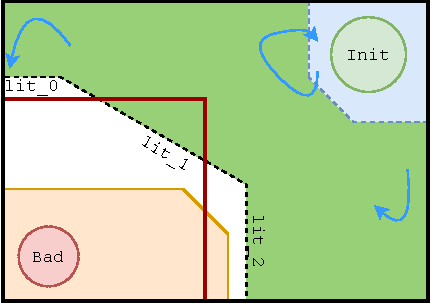
\includegraphics[width=0.99\textwidth]{figures/doping-lemma.pdf}
    \caption{An inductive lemma L = \{\texttt{lit\_0}, \texttt{lit\_1}, \texttt{lit\_2}\}}
    \label{fig:lemma}
	\end{subfigure}
	\begin{subfigure}[b]{0.3\textwidth}
    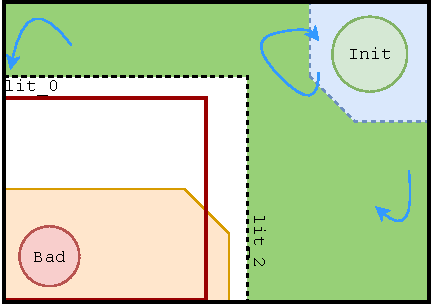
\includegraphics[width=0.99\textwidth]{figures/doping-lemma_gen.pdf}
    \caption{L is successfully generalized by dropping \texttt{lit\_1}}
    \label{fig:ind_gen}
	\end{subfigure}
	\begin{subfigure}[b]{0.3\textwidth}
    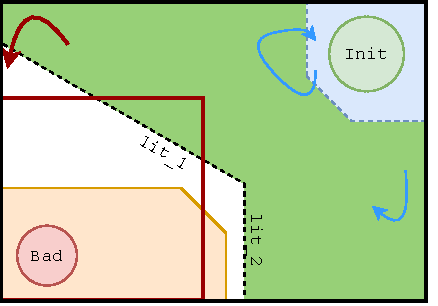
\includegraphics[width=0.99\textwidth]{figures/doping-lemma_not_ind.pdf}
    \caption{L no longer inductive by dropping \texttt{lit\_0}}
    \label{fig:not_ind_gen}
	\end{subfigure}

  \caption{Visualization of inductive generalization.}
  \label{fig:vis_ind_gen}
\end{figure*}




\paragraph{IC3/\spc.}
The current state-of-the-art algorithm to solve CHC is IC3/\spc \cite{spacer}.
At the high level, the main IC3/\spc loop will try to find a CEX of length $N$,
and terminate if the CEX is found (\unsafe), or the lemma that proves such CEX
doesn't exist is also a safe inductive invariant (\safe). 

There are many ways to represent \spc algorithm, and in this thesis we borrows
the presentation used in \cite{GSpacer}.

\cref{alg:spc} presents the key ingredients of \spc as a set of rules. It
maintains the following.
\begin{itemize}
  \item Current unrolling depth $N$ at
    which a counterexample is searched (there are no counterexamples with depth less
    than $N$).
  \item An inductive trace $F = [F_0, F_1, \ldots]$.
    Intuitively, each frame $F_i$ is a candidate inductive invariant s.t.
    $F_i$ over-approximates states reachable up to $i$ steps from $\Init$.

  \item A queue of \emph{proof obligations} $Q$, where each proof obligation
    (\pob) in $Q$ is a pair $\langle \varphi, i \rangle$ of a cube $\varphi$ and a
    level number $i$, $0 \leq i \leq N$.
    Each \pob $\langle \varphi, i \rangle$ in $Q$ corresponds to a suffix of a potential
    counterexample that has to be blocked in $F_i$, i.e., has to be proven unreachable in $i$ steps.
  \item An under-approximation $\cU$ of reachable
    states, represented as a disjunction.
\end{itemize}


% \spc maintains the following data structures:
% \begin{itemize}
%     \item A unrolling depth $N$
%     \item An under-approximation $U$ of reachable states
%     \item  A queue of \emph{proof obligations} $Q$, where each proof obligation (\pob) in $Q$ is a pair $\langle \varphi, i \rangle$ of a cube $\varphi$ and a level number $i$, $0 \leq i \leq N$. Each POB is a region containing a potential counterexample that we want to prove to be unreachable (blocked) in $i$ steps.
%     \item A trace of frames $F$, in which each frame $F_i$ is a set of lemmas. Intuitively, each frame $F_i$ over-approximates states reachable up to $i$ steps from $\Init$. A lemma is learnt when a POB is blocked. Intuitively, a lemma is a region containing the reachable states but not the POB (the green region if Fig \ref{fig:ind_gen}, 
% \end{itemize}
% At the high level, the main IC3/\spc loop will try to find a counterexample of length $N$, and terminate if the counterexample is found (UNSAFE), or the lemma that proves such counterexample doesn't exist is a safe inductive invariant(SAFE). 

% The \texttt{Candidate} rule adds an initial \pob $\langle \Bad, N \rangle$ to
% the queue. If a \pob $\langle \varphi, i \rangle$ cannot be blocked because
% $\varphi$ is reachable from frame $(i-1)$, the \texttt{Predecessor} rule
% generates a predecessor $\psi$ of $\varphi$ using MBP and adds $\langle \psi,
% i-1 \rangle$ to $Q$. The \texttt{Successor} rule updates the set of reachable
% states if the \pob is reachable. If the \pob is blocked, the \texttt{Conflict}
% rule strengthens the trace $F$ by using interpolation to learn a new lemma
% $\ell$ that blocks the \pob, i.e., $\ell$ implies $\neg \varphi$. The
% \texttt{Induction} rule strengthens a lemma by inductive generalization and the
% \texttt{Propagate} rule pushes a lemma to a higher frame. If the $\Bad$ state
% has been blocked at $N$, the \texttt{Unfold} rule increments the depth of
% unrolling $N$. In practice, the rules are scheduled to ensure progress towards
% finding a counterexample.\DecMargin{0.1in}




% The main data structure in \spc is a queue of proof obligation $Q$, and 

% \cref{alg:spc} presents the key ingredients of \spc as a set of guarded
% commands (or rules). It maintains the following. Current unrolling depth $N$ at
% which a counterexample is searched (there are no counterexamples with depth less
% than $N$). A \emph{trace} $F = (F_0, F_1, \ldots)$ of \emph{frames}, such that
% each frame $F_i$ is a set of \emph{lemmas}, and each lemma $\ell \in F_i$ is
% a clause.
%  A queue of \emph{proof obligations} $Q$, where each proof obligation
% (\pob) in $Q$ is a pair $\langle \varphi, i \rangle$ of a cube $\varphi$ and a
% level number $i$, $0 \leq i \leq N$. An under-approximation $\cU$ of reachable
% states. Intuitively, each frame $F_i$ is a candidate inductive invariant s.t.
% $F_i$ over-approximates states reachable up to $i$ steps from $\Init$.
% The latter is ensured since $F_0 = \Init$, the trace is monotone, i.e.,
% $F_{i+1} \subseteq F_i$, and each frame is inductive \emph{relative} to its previous one,
% i.e., $F_i \wedge \Tr \limp F_{i+1}'$.
% Each \pob $\langle \varphi, i \rangle$ in $Q$ corresponds to a suffix of a potential
% counterexample that has to be blocked in $F_i$, i.e., has to be proven unreachable in $i$ steps.



% The \texttt{Candidate} rule adds an initial \pob $\langle \Bad, N \rangle$ to
% the queue. If a \pob $\langle \varphi, i \rangle$ cannot be blocked because
% $\varphi$ is reachable from frame $(i-1)$, the \texttt{Predecessor} rule
% generates a predecessor $\psi$ of $\varphi$ using MBP and adds $\langle \psi,
% i-1 \rangle$ to $Q$. The \texttt{Successor} rule updates the set of reachable
% states if the \pob is reachable. If the \pob is blocked, the \texttt{Conflict}
% rule strengthens the trace $F$ by using interpolation to learn a new lemma
% $\ell$ that blocks the \pob, i.e., $\ell$ implies $\neg \varphi$. The
% \texttt{Induction} rule strengthens a lemma by inductive generalization and the
% \texttt{Propagate} rule pushes a lemma to a higher frame. If the $\Bad$ state
% has been blocked at $N$, the \texttt{Unfold} rule increments the depth of
% unrolling $N$. In practice, the rules are scheduled to ensure progress towards
% finding a counterexample.\DecMargin{0.1in}


 


% Given a lemma in cube form $\cC$, its semantic meaning is that the system is safe at some state $\cS$ because of $\cC$. By dropping some of the literals in $\cC$, we ... 
% \nl{remember to add an example}

% The loop invariant is built within the given context of program. Thus it is natural to encode the program
% as an external memory module. However, in contrast to traditional memory networks [19, 20], where
% the memory slots are organized as a linear array, the information contained in a program has rich
% structure. A chain LSTM over program tokens can in principle capture such information but it is
% challenging for neural networks to understand with limited data. Inspired by Allamanis et al. [21], we
% instead use a graph-structured memory representation. Such a representation allows to capture rich
% semantic knowledge about the program such as its control-flow and data-flow

%%% Local Variables:
%%% mode: latex
%%% TeX-master: "0.0_main"
%%% End:


The \texttt{Candidate} rule adds a \pob $\langle \Bad, N \rangle$ to
the queue. If a \pob $\langle \varphi, i \rangle$ cannot be blocked because
$\varphi$ is reachable from frame $(i-1)$, the \texttt{Predecessor} rule
generates a predecessor $\psi$ of $\varphi$ using \getP, and add $\langle \psi,
i-1 \rangle$ to $Q$. The \texttt{Successor} rule updates the set of reachable
states if the \pob is reachable. If the \pob is blocked, the \texttt{Conflict}
rule strengthens the trace $F$ by using interpolation to learn a new lemma
$\ell$ that blocks the \pob, i.e., $\ell \implies \neg \varphi$. The
\texttt{Induction} rule strengthens a lemma by inductive generalization and the
\texttt{Propagate} rule pushes a lemma to a higher frame. If the $\Bad$ state
has been blocked at $N$, the \texttt{Unfold} rule increments the depth of
unrolling $N$. In practice, the rules are scheduled to ensure progress towards
finding a counterexample.
\begin{algorithm2e}[t]
  \SetAlgoNoLine
  \LinesNotNumbered
  \SetKwIF{Guard}{Guard1}{Guard2}{$[$}{$]$}{}{}{}
  \SetKwComment{Rule}{}{}
  \SetKwFor{select}{forever do}{}{}
  \Fn{\spc}{
    \Indm
    \KwIn{$\langle \Init, \Tr, \Bad \rangle$}
    \KwOut{$\langle \safe, \Inv \rangle$ or \unsafe}
    $Q := \emptyset$ \tcp*{\pob queue}
    $N := 0$ \tcp*{maximum safe level}
    $F_0 := \Init, F_i := \top \textbf{ for all } i > 0$ \tcp*{lemma trace}
    $\cU := \Init$ \tcp*{reachable states}
    \select{}{
      \Rule*[h]{Candidate} \lGuard {$\isSat(F_N \land \Bad)$} {
        
        $\qquad Q := Q \cup
        \langle \Bad, N \rangle$}

      \Rule*[h]{Predecessor} \lGuard {$\langle \varphi, i + 1 \rangle \in Q$, $M \models
        F_i \land \Tr \land \varphi'$}{

        $\qquad Q := Q \cup \langle \getP(\varphi, M), i \rangle$}


      \Rule*[h]{Successor} \lGuard {$\langle \varphi, i + 1 \rangle \in Q$, $M \models \cF(\cU) \land
        \varphi'$}{

        $\qquad \cU := \cU \lor  \getS(\cU, M)[\Consts' \mapsto\Consts]$}

      \Rule*[h]{Conflict} \lGuard {$\langle \varphi, i + 1 \rangle \in Q$, $\cF(F_i) \limp \neg \varphi'$}
      {

        $\qquad F_j := ( F_j \land  \itp(\cF(F_i), \varphi')[\Consts' \mapsto \Consts] )
        \makebox[0pt][l]{ $\textbf{ for all } j \leq i + 1 $}$}

      \Rule*[h]{Induction} \lGuard{$\ell \in F_{i+1}, \ell = (\varphi \lor \psi), \cF(\varphi \land F_i) \limp
        \varphi'$}{

        $\qquad F_{j} \gets F_{j} \land \varphi \textbf{ for all } j
        \leq i + 1$}

      \Rule*[h]{Propagate} \lGuard{$\ell \in F_{i}, F_i \land \Tr \limp
        \ell'$}{

        $\qquad F_{i + 1} \gets (F_{i + 1} \land \ell)$}

      \Rule*[h]{Unfold} \lGuard {$F_N \limp \neg \Bad$}{

        $\qquad N := N + 1$}

      \Rule*[h]{Safe} \lGuard {$F_{i + 1} \limp F_{i} {\normalfont \textbf{ for some }} i <
        N$}{

        \qquad \Return $\langle  \safe, F_i \rangle$}

      \Rule*[h]{Unsafe} \lGuard {\isSat($\Bad \land \cU$)}{

        \qquad \Return \unsafe}
    }
  }
  \caption{\spc algorithm as described in \cite{GSpacer}, modified to make
    annotation coherent. $\Consts$ and $\Consts'$ are constant symbols, which
    typically represent program variables. We use the shorthand $\cF(\varphi) = \cU' \lor (\varphi \land \Tr)$.}
  \label{alg:spc}
\end{algorithm2e}

\paragraph{Inductive generalization}
The \texttt{Induction} rule is a crucial optimization to IC3. To block a \pob
$\varphi$, it is enough to learn the clause $\lnot \varphi$. However, most of the
time, this clause is too weak to block any other \pob. As illustrated in
\cref{fig:lemma}, to block the orange \pob, we can learn the lemma
${lit_0, lit_1, lit_2}$ (slightly shifted because of the interpolation). This
lemma is too weak, and cannot be used to block the red-lined \pob. Since there
could be exponentially many \pobs, it is of the utmost importance that a learned
lemma could be reused to block multiple \pobs. One way to do so is to try to
drop literals in the learned lemma, and check that the reduced lemma is still
inductive relative to the previous frame.
As we can see from \cref{fig:not_ind_gen}, starting from the lemma $\{\texttt{lit\_0}, \texttt{lit\_1}, \texttt{lit\_2}\}$, dropping \texttt{lit\_0} results in a lemma that is no longer inductive, while dropping \texttt{lit\_1} doesn't affect its inductiveness, as illustrated in \cref{fig:ind_gen}.

